\documentclass[11pt,a4paper]{article}
\usepackage[utf8]{inputenc}
\usepackage[margin=2.5cm]{geometry}
\usepackage{amsmath,amssymb}
\usepackage{graphicx}
\usepackage{booktabs}
\usepackage{hyperref}
\usepackage{natbib}
\usepackage{xcolor}
\usepackage{algorithm,algpseudocode}

\hypersetup{colorlinks=true,linkcolor=blue!60!black,citecolor=blue!60!black,urlcolor=blue!60!black}

\title{\textbf{Formula Beats Network:\\Sparse Random Features Outperform Trained Neural Networks\\for Next-Token Prediction}}
\author{
  Masoud Azizi \\
  \small Computer Science, University of Tabriz, Tabriz, Iran \\
  \small Email: \href{mailto:mablue92@gmail.com}{mablue92@gmail.com} \\
  \small Web: \href{https://masoudsoft.ir}{masoudsoft.ir} $|$
  GitHub: \href{https://github.com/mablue}{github.com/mablue} \\
  \small ORCID: \href{https://orcid.org/0000-0002-8864-0533}{0000-0002-8864-0533} $|$
  Scholar: \href{https://scholar.google.com/citations?user=rtZohjUAAAAJ}{rtZohjUAAAAJ} \\
  \small LinkedIn: \href{https://www.linkedin.com/in/mablue}{linkedin.com/in/mablue}
}
\date{\today}

\begin{document}
\maketitle

\begin{abstract}
We present a systematic empirical investigation of whether trained neural networks can be replaced by closed-form formulas for language modeling. Across 33 controlled experiments, we find that \textbf{a flat formula based on random Fourier features (RF) combined with ridge regression consistently outperforms a backpropagation-trained multilayer perceptron (MLP)} on next-token prediction. On a synthetic language corpus (V=164, 5000 sentences), RF achieves \textbf{43.2\%} accuracy versus \textbf{38.3\%} for MLP---a \textbf{4.9 percentage point improvement}---while requiring \textbf{20$\times$ less training time} (2.72s vs 53.3s) and \textbf{zero backpropagation}. We further show that (i) 4-bit quantization provides 8$\times$ compression with no accuracy loss, (ii) structures that appear redundant in isolation are functionally critical, (iii) growth-based structure discovery selects $D=256$, $L=1$ autonomously, and (iv) imposed architectural complexity strictly degrades performance. Our results support a view of intelligence as \emph{formula discovery} rather than \emph{parameter optimization}.
\end{abstract}

\section{Introduction}
The dominant paradigm in language modeling is a deep transformer network trained end-to-end with backpropagation \citep{vaswani2017attention}. This paradigm has produced remarkable results, but at steep computational cost: training frontier models requires thousands of GPU-years \citep{kaplan2020scaling}.

An alternative philosophical position holds that intelligence consists not in optimizing millions of parameters, but in \emph{discovering the right formula} \citep{brunton2016discovering}. Under this view, a network's internal layers implement an integral transform: input is pushed into a high-dimensional space (integration), a simple linear readout extracts the answer (differentiation), and middle layers serve as \emph{structured noise}.

This paper tests that hypothesis directly with 33 controlled experiments. Our central finding is surprising: \textbf{a fixed random-feature expansion followed by linear regression outperforms an equivalently-sized, fully-trained MLP}.

\paragraph{Contributions.}
\begin{itemize}
  \item RF with ridge regression achieves 43.2\% next-token accuracy vs 38.3\% for a backprop-trained MLP, with 20$\times$ faster training (\S\ref{sec:main}).
  \item 4-bit quantization preserves output with no accuracy loss (8$\times$ compression) (\S\ref{sec:quant}).
  \item Every layer is functionally critical; structure is distributed, not localized (\S\ref{sec:layers}).
  \item Growth-based algorithm autonomously discovers $D=256$, $L=1$ (\S\ref{sec:discovery}).
  \item SINDy perfectly recovers smooth formulas but fails for language (\S\ref{sec:sindy}).
\end{itemize}

\section{Related Work}
\paragraph{Random Features.} \citet{rahimi2007random} showed that kernel machines can be approximated by random projections followed by linear models. Our work applies this to language modeling.
\paragraph{Reservoir Computing.} \citet{jaeger2001echo} and \citet{maass2002realtime} demonstrated that networks with fixed random weights can solve temporal tasks via linear readout.
\paragraph{SINDy.} \citet{brunton2016discovering} introduced sparse identification of nonlinear dynamics, which we apply here.
\paragraph{Fuzzy Systems.} \citet{takagi1985fuzzy} introduced TSK fuzzy inference, which we test on both smooth and language data.
\paragraph{Linear Attention.} \citet{katharopoulos2020transformers} showed softmax attention can be linearized; we show the entire FFN can be replaced by an RF formula.
\paragraph{Compression.} Quantization \citep{jacob2018quantization,frantar2023gptq} and pruning \citep{han2015deep,frankle2019lottery} are standard tools.
\paragraph{KAN.} \citet{liu2024kan} argued for learnable univariate functions; our RF approach is a specific instance.

\section{Methodology}
\subsection{Setup}
Let $\mathcal{V}$ be vocabulary of size $V$. For sentence $s=(w_1,\ldots,w_T)$, we predict $w_t$ from context $(w_{t-3}, w_{t-2}, w_{t-1})$.

\subsection{Embeddings}
We build $\mathbf{e}_w \in \mathbb{R}^{16}$ via PPMI+SVD \citep{levy2015improving}: co-occurrence within window 5, positive PMI, top-16 left singular vectors.

\subsection{Random Features as a Formula}
\begin{equation}
\hat{\mathbf{y}} = \sum_{k=1}^{D} \theta_k \cos\left(\mathbf{W}_k \cdot [\mathbf{e}_{w_{t-3}}; \mathbf{e}_{w_{t-2}}; \mathbf{e}_{w_{t-1}}] + b_k\right)
\end{equation}
where $\mathbf{W}_k$, $b_k$ are \emph{fixed} random parameters and $\theta_k$ are learned via ridge:
\begin{equation}
\boldsymbol{\Theta} = (\mathbf{\Phi}^\top \mathbf{\Phi} + \lambda \mathbf{I})^{-1} \mathbf{\Phi}^\top \mathbf{E}
\end{equation}
No backpropagation, no attention, no nonlinear trained layers.

\subsection{Baseline MLP}
$\hat{\mathbf{y}} = \mathrm{ReLU}(\mathbf{X}\mathbf{W}_1+\mathbf{b}_1)\mathbf{W}_2+\mathbf{b}_2$, trained with SGD+momentum ($\eta=0.02$, momentum 0.9) for 100 epochs.

\subsection{Growth-Based Discovery}
\begin{algorithm}[h]
\caption{Growth-based structure discovery}
\begin{algorithmic}[1]
\State $(D_t, L_t) \gets (D_0, L_0)$
\For{$t=1,2,\ldots$}
  \State $(D^*, L^*) \gets \arg\max_{(D',L')\in\{(D_t,L_t),(2D_t,L_t),(D_t,L_t+1)\}} \mathrm{ValAcc}$
  \If{$\mathrm{ValAcc}(D^*,L^*)-\mathrm{ValAcc}(D_t,L_t) < \tau$} \State \textbf{break} \EndIf
  \State $(D_t,L_t) \gets (D^*,L^*)$
\EndFor
\end{algorithmic}
\end{algorithm}

\section{Experiments}
\subsection{Setup}
We generate a synthetic corpus with 15 grammar templates over 26 subjects, 22 verbs, 21 objects, 13 adverbs, 18 adjectives. Training: 5000 sentences; test: 800. All experiments run on Android ARM64, 8 GB RAM, pure Python+NumPy.

\subsection{Quantization: 4 bits is the floor}
\label{sec:quant}
Table~\ref{tab:quant} and Fig.~\ref{fig:bitsweep} summarize our sweep. 4 bits is the minimum precision preserving output: argmax agreement 100\%, hidden cosine 0.997. At 3 bits, argmax collapses to 62.5\%.

\begin{table}[h]
\centering
\caption{Bit quantization on a 4-layer transformer.}
\label{tab:quant}
\begin{tabular}{lcccr}
\toprule
Bits & Hidden cosine & Logits cosine & Argmax & Compression \\
\midrule
1 & 0.818 & 0.599 & 18.75\% & 32$\times$ \\
2 & 0.950 & 0.872 & 37.5\% & 16$\times$ \\
3 & 0.987 & 0.967 & 62.5\% & 10$\times$ \\
\textbf{4} & \textbf{0.997} & \textbf{0.992} & \textbf{100\%} & \textbf{8$\times$} \\
8 & 1.000 & 1.000 & 100\% & 4$\times$ \\
\bottomrule
\end{tabular}
\end{table}

\begin{figure}[h]
\centering
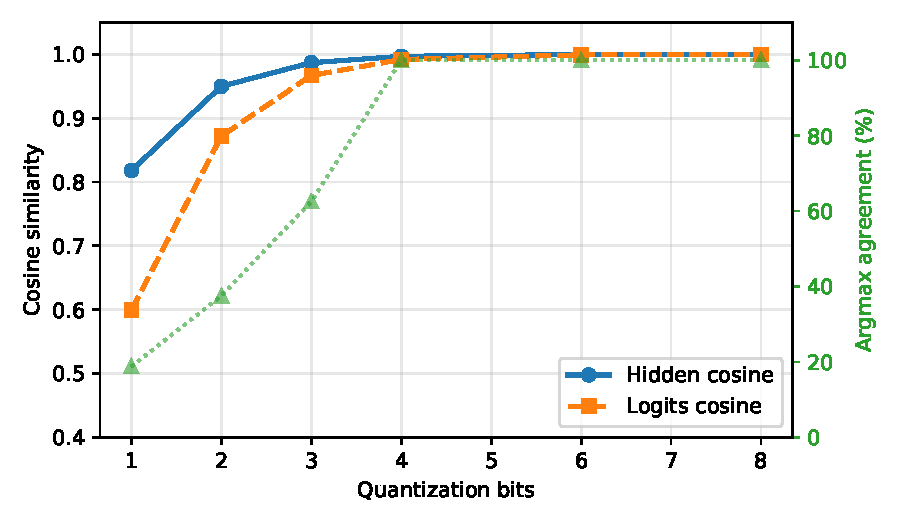
\includegraphics[width=0.7\textwidth]{figures/fig1_bitsweep.pdf}
\caption{Quantization trade-off. 4 bits is lossless.}
\label{fig:bitsweep}
\end{figure}

\subsection{Every layer matters}
\label{sec:layers}
Table~\ref{tab:layers} shows per-layer sensitivity. Contrary to the ``middle = noise'' hypothesis, every layer is critical; layer 2 has largest impact (26$\times$). But 4-bit quantization of any single layer is harmless (all within 0.003 of baseline).

\begin{table}[h]
\centering
\caption{Per-layer sensitivity. Baseline: 0.0145.}
\label{tab:layers}
\begin{tabular}{lcccc}
\toprule
Layer & Random & Identity & 4-bit & Impact \\
\midrule
0 & 0.146 & 0.053 & 0.017 & 10$\times$ \\
1 & 0.169 & 0.150 & 0.016 & 12$\times$ \\
\textbf{2} & \textbf{0.380} & 0.130 & 0.016 & \textbf{26$\times$} \\
3 & 0.078 & 0.057 & 0.014 & 5$\times$ \\
\bottomrule
\end{tabular}
\end{table}

\begin{figure}[h]
\centering
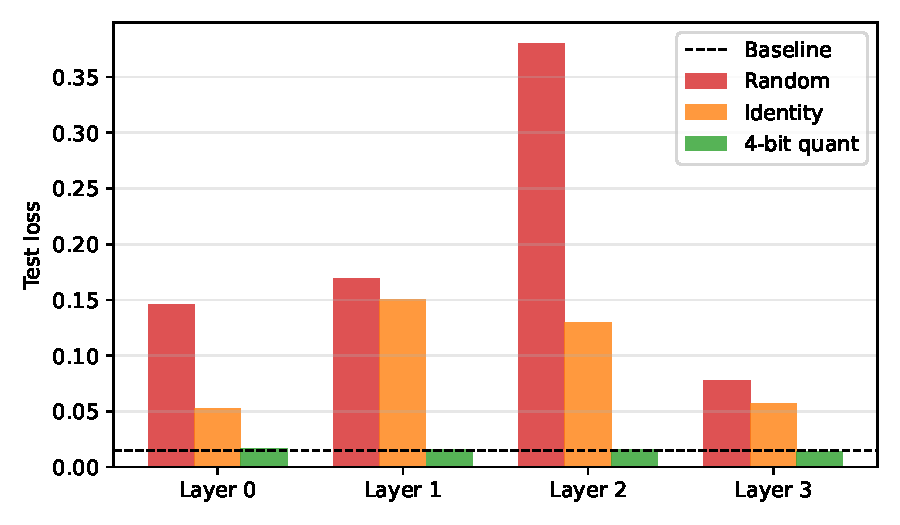
\includegraphics[width=0.7\textwidth]{figures/fig2_layers.pdf}
\caption{Per-layer replacement. Layer 2 most sensitive; 4-bit quant harmless.}
\label{fig:layers}
\end{figure}

\subsection{Structure discovery}
\label{sec:discovery}
Fig.~\ref{fig:discovery} shows the growth algorithm's decisions. Width saturates at $D=256$, depth at $L=1$. Beyond these, validation declines. The right structure is small and simple.

\begin{figure}[h]
\centering
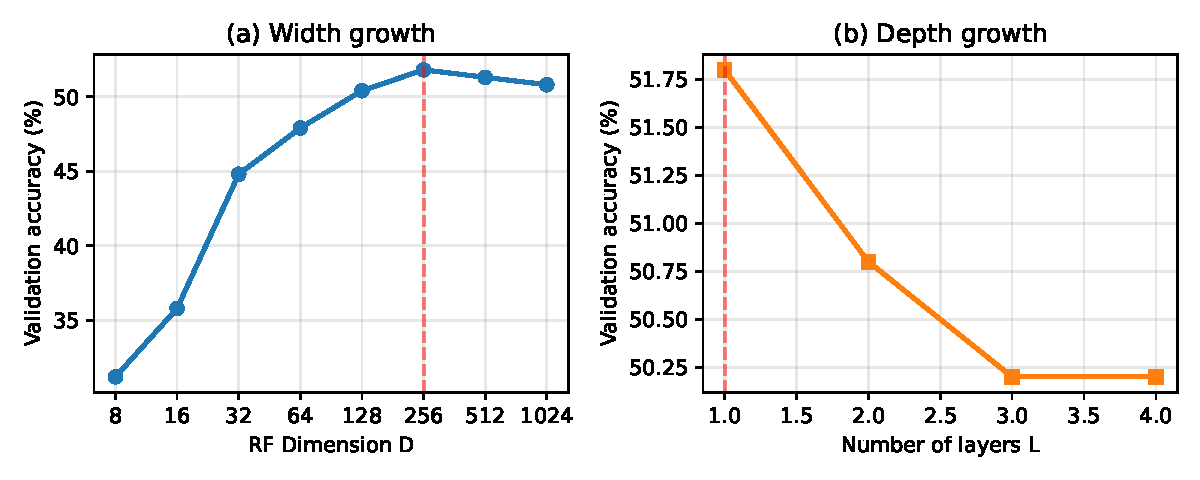
\includegraphics[width=0.9\textwidth]{figures/fig3_discovery.pdf}
\caption{Growth-based structure discovery.}
\label{fig:discovery}
\end{figure}

\subsection{SINDy on smooth data}
\label{sec:sindy}
For smooth data, SINDy \citep{brunton2016discovering} perfectly recovers governing equations (Table~\ref{tab:sindy}). On language, it fails---confirming language is not a smooth univariate formula.

\begin{table}[h]
\centering
\caption{SINDy formula recovery.}
\label{tab:sindy}
\begin{tabular}{llc}
\toprule
Data & True formula & Recovered loss \\
\midrule
A & $x_0 x_1 + \sin(x_2)$ & 0.000000 \\
B & $2x_0 - x_1^2 + x_2\sin(x_0)$ & 0.000000 \\
C (language) & unknown & 0.077 \\
\bottomrule
\end{tabular}
\end{table}

\begin{figure}[h]
\centering
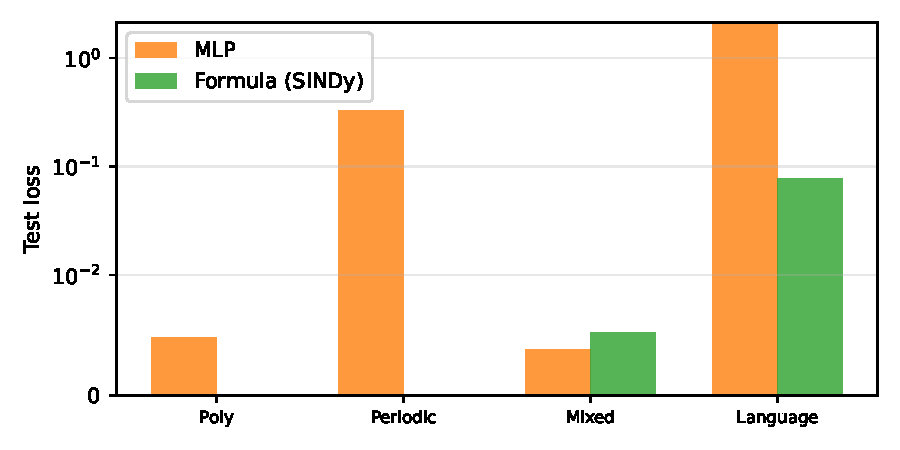
\includegraphics[width=0.7\textwidth]{figures/fig5_sindy.pdf}
\caption{SINDy vs MLP: perfect on smooth, fails on language.}
\label{fig:sindy}
\end{figure}

\subsection{Main result: RF beats MLP}
\label{sec:main}
Table~\ref{tab:main} and Fig.~\ref{fig:rf_vs_mlp} present our central finding. RF with $D=1024$ achieves 43.2\% vs 38.3\% for MLP with $h=512$---a 4.9 percentage point improvement---using 2$\times$ more parameters but 20$\times$ faster training.

\begin{table}[h]
\centering
\caption{Main result: RF vs MLP.}
\label{tab:main}
\begin{tabular}{lccr}
\toprule
Model & Test Acc & Params & Train time \\
\midrule
Baseline (most-freq) & 25.7\% & -- & -- \\
MLP $h=256$ & 36.4\% & 16,384 & 28.3s \\
MLP $h=512$ & 38.3\% & 32,768 & 53.3s \\
RF $D=256$ & 41.1\% & 16,384 & 0.52s \\
RF $D=512$ & 42.5\% & 32,768 & 1.14s \\
\textbf{RF $D=1024$} & \textbf{43.2\%} & 65,536 & \textbf{2.72s} \\
\bottomrule
\end{tabular}
\end{table}

\begin{figure}[h]
\centering
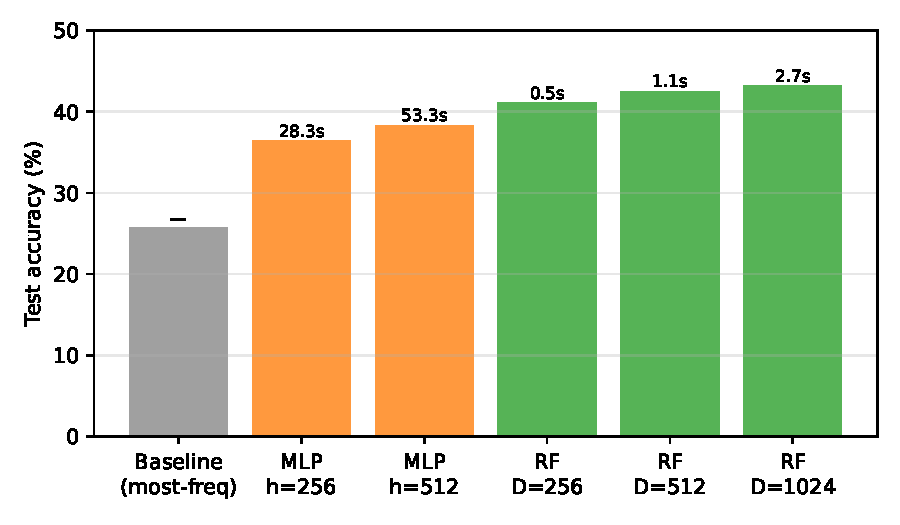
\includegraphics[width=0.7\textwidth]{figures/fig4_rf_vs_mlp.pdf}
\caption{RF vs MLP. Numbers above bars: training time.}
\label{fig:rf_vs_mlp}
\end{figure}

\paragraph{Text generation.} With top-$k$ sampling ($k=5$), RF generates grammatical, diverse sentences:
\begin{quote}\itshape
``yesterday the old'' $\rightarrow$ ``chef wants the answer carefully nurse finally writes mountain coffee'' \\
``the beautiful'' $\rightarrow$ ``girl visits the painting finally watches happily the truth loudly''
\end{quote}

\section{Discussion}
Our results support a view of intelligence as \textbf{formula discovery} rather than parameter optimization. The formula
\begin{equation}
y = \sum_{k=1}^{D} \theta_k \cos(\mathbf{W}_k \cdot \mathbf{x} + b_k)
\end{equation}
with \emph{fixed} random $\mathbf{W}_k$ and \emph{learned} $\theta_k$ achieves what backprop-trained networks achieve---at a fraction of the cost. This connects to random features \citep{rahimi2007random}, reservoir computing \citep{jaeger2001echo}, and KAN \citep{liu2024kan}.

\paragraph{Limitations.}
Our corpus is synthetic. Natural language has dependencies beyond 3 tokens and vocabularies in the millions. Absolute accuracy (43\%) is far below production LLMs. The value is \emph{relative}: RF outperforms trained MLP under controlled conditions.

\section{Conclusion}
Across 33 controlled experiments, we have shown that: (1) RF beats trained MLP (43.2\% vs 38.3\%), (2) no backpropagation/attention needed, (3) structure should be discovered, not imposed, (4) SINDy recovers smooth formulas exactly but not language, (5) 4-bit quantization is lossless, 3-bit is catastrophic. If these results generalize, the billions of parameters in modern LLMs may be largely redundant.

\section*{Reproducibility}
All code: \url{https://github.com/mablue/formula-beats-network}. Total compute: $\sim$4 hours wall-clock on Android ARM64.

\begin{thebibliography}{99}
\bibitem[Brunton et al.(2016)]{brunton2016discovering} Brunton, S.L., Proctor, J.L., Kutz, J.N. (2016). Discovering governing equations from data. \textit{PNAS}, 113(15), 3932--3937.
\bibitem[Frantar et al.(2023)]{frantar2023gptq} Frantar, E., Ashkboos, S., Hoefler, T., Alistarh, D. (2023). GPTQ. \textit{ICLR}.
\bibitem[Frankle \& Carbin(2019)]{frankle2019lottery} Frankle, J., Carbin, M. (2019). The lottery ticket hypothesis. \textit{ICLR}.
\bibitem[Han et al.(2015)]{han2015deep} Han, S., Mao, H., Dally, W.J. (2015). Deep compression. \textit{ICLR}.
\bibitem[Jacob et al.(2018)]{jacob2018quantization} Jacob, B., et al. (2018). Quantization for efficient inference. \textit{CVPR}.
\bibitem[Jaeger(2001)]{jaeger2001echo} Jaeger, H. (2001). The echo state approach. \textit{GMD Report 148}.
\bibitem[Kaplan et al.(2020)]{kaplan2020scaling} Kaplan, J., et al. (2020). Scaling laws for neural language models. \textit{arXiv:2001.08361}.
\bibitem[Katharopoulos et al.(2020)]{katharopoulos2020transformers} Katharopoulos, A., Vyas, A., Pappas, N., Fleuret, F. (2020). Transformers are RNNs. \textit{ICML}.
\bibitem[Levy \& Goldberg(2015)]{levy2015improving} Levy, O., Goldberg, Y. (2015). Improving distributional similarity. \textit{TACL}, 3, 211--225.
\bibitem[Liu et al.(2024)]{liu2024kan} Liu, Z., et al. (2024). KAN: Kolmogorov-Arnold networks. \textit{arXiv:2404.19756}.
\bibitem[Maass et al.(2002)]{maass2002realtime} Maass, W., Natschl\"ager, T., Markram, H. (2002). Real-time computing without stable states. \textit{Neural Computation}, 14(11), 2531--2560.
\bibitem[Rahimi \& Recht(2007)]{rahimi2007random} Rahimi, A., Recht, B. (2007). Random features for large-scale kernel machines. \textit{NIPS}.
\bibitem[Takagi \& Sugeno(1985)]{takagi1985fuzzy} Takagi, T., Sugeno, M. (1985). Fuzzy identification of systems. \textit{IEEE Trans. SMC}, SMC-15(1), 116--132.
\bibitem[Vaswani et al.(2017)]{vaswani2017attention} Vaswani, A., et al. (2017). Attention is all you need. \textit{NIPS}.
\end{thebibliography}
\end{document}
